\chapter{Analiza wyników, możliwe drogi dalszych badań}\label{chap:results_analysis}


% Wyniki uzyskane przez zaimplementowany algorytm optymalizacji
% opisane w rozdziałach~\ref{chap:research} oraz~\ref{target_function_chapter} pozwalają

Wyniki przedstawione w rozdziałach~\ref{chap:research} oraz~\ref{target_function_chapter}
wskazują, że zaimplementowany algorytm optymalizacji wytwarza poprawne rozwiązania
dla części problemów. Nawet gdy finalnie wygenerowane brzmienie różni
się od dźwięku docelowego, algorytm wytwarza interesujące barwy dźwięku,
które można zakwalifikować jako~,,wariacje'' na temat oryginalnego sygnału.
Tego typu wyniki mogą być wartościowe dla potencjalnych użytkowników algorytmu.
W niniejszym rozdziale przeprowadzono szczegółową analizę obserwacji,
uzyskanych podczas procesu badawaczego.


\section{Zbiór danych testowych}\label{sec:not_enough_benchmarking_data}

Automatyczna konstrukcja elektronicznych instrumentów muzycznych jest stosunkowo
nowym obszarem badań, w związku z czym brakuje odpowiednich zbiorów danych
umożliwiających porównywanie sprawności różnych algorutmów.
Porównanie wykonane w niniejszej pracy nie stanowi przekroju
przez wiele możliwych typów syntezy, ponieważ w procesie przeglądu
literatury nie udało się znaleźć stosownego zbioru danych.

Jak pokazały wyniki opisane w sekcji~\ref{sec:non_literature_samples},
zaimplementowany algorytm generuje lepsze rozwiązania w przypadku
syntezy \textit{analog modeling}, podczas gdy praca służąca
za porównanie~\cite{evolutionary_puredata} zawiera głownie przykłady
syntezy FM oraz nagrania instrumentów dętych. Sugestie dotyczące
stworzenia bardziej różnorodnego zbioru dźwięków o różnych barwach
i dynamice zawarto w sekcji~\ref{sec:potential_improvements}.


\section{Optymalizacja parametrów grafu dla problemów o małej złożoności}

Jak wykazały testy przeprowadzone w rozdziale~\ref{target_function_chapter},
zaimplementowany algorytm jest w stanie dokładnie odtworzyć wartości
parametrów grafu dla prostych problemów syntezy
FM~(\ref{fig:param_optimisation_results_spectrograms})
i umiarkowanie złożonych problemów syntezy
\textit{analog modeling}~(\ref{fig:am_param_optimisation_results_spectrograms}).
Testy na małej próbie słuchaczy pozwalają stwierdzić,
że \textbf{nie są oni w stanie odróżnić} sygnałów wygenerowanych
dla problemów z rozdziału~\ref{target_function_chapter}
od dźwięków docelowych.

% \begin{enumerate}
%   \item Nawet jak nie działa to idzie w kierunku celu, często generując interesujące brzmienia po drodze,
%   \item Problemy ze zmianami w dynamice, szczególnie pierwsze ułamki sekund,
% \end{enumerate}


\section{Potencjał wykorzystania w przemyśle muzycznym}

Wytwarzane przez algorytm barwy są zróżnicowane i brzmią
w sposób~,,muzyczny'' -- nawet gdy wygenerowany dźwięk
znacząco różni się od docelowej barwy, algorytm nie generuje
szumu ani~,,kakofonii''. 
Zaimplementowany algorytm może być uruchomiony na standardowym komputerze,
dostępnym dla przeciętnego użytkownika, co otwiera możliwość jego integracji
z oprogramowaniem typu \textit{digital audio workstation}. Integracja
z oprogramowaniem do produkcji muzyki otwiera drogę do wykorzystania
wtyczek \texttt{VST}, znacznie zwiększając liczbę dostępnych
dla algorytmu węzłów przetwarzania sygnału, potencjalnie usprawniając
jego działanie.


\section{Potencjalne usprawnienia wydajności algorytmu}

\begin{figure}[H]
    \centering
    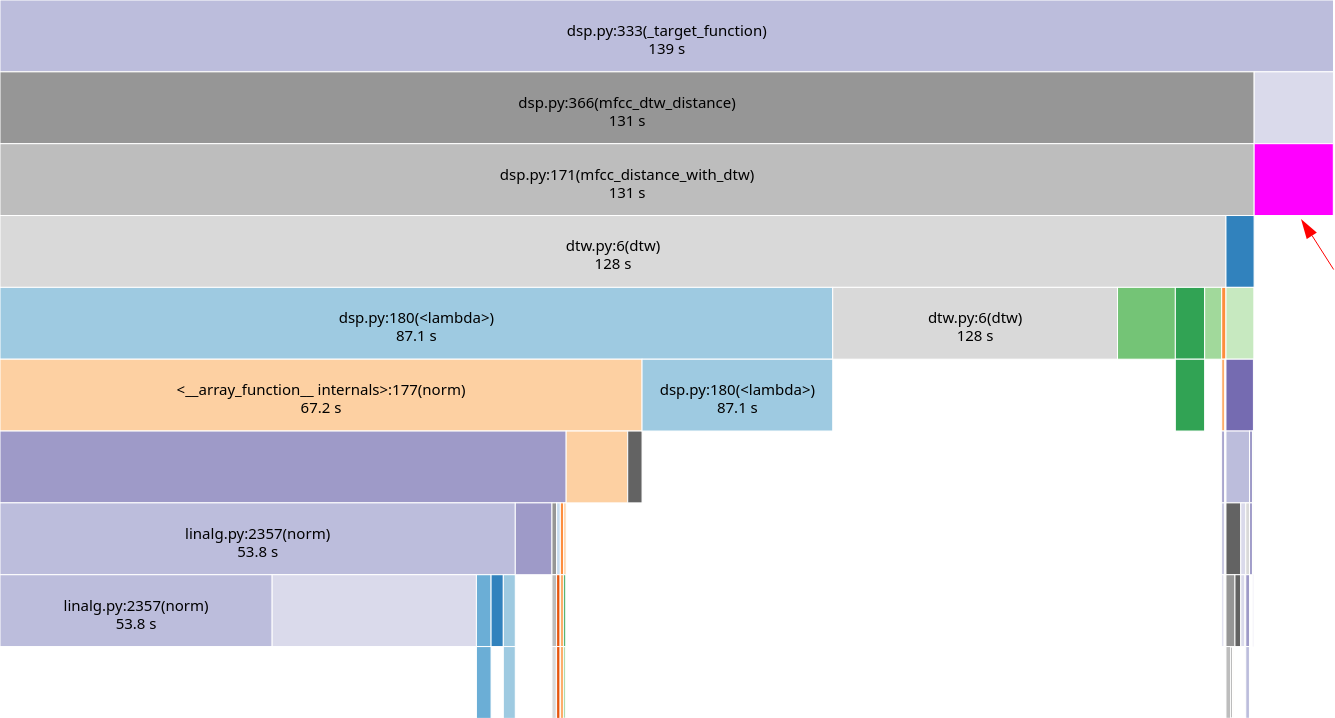
\includegraphics[width=1.0\linewidth]{rys07/profile_target_function_execution.png}
    \caption{
      Wizualizacja danych wygenerowanych przez profiler języka Python
      dla przykładowego problemu optymalizacji. Widoczne składowe wpływające
      na sumaryczny czas ewaluacji funkcji celu.
      Czerwoną strzałką oznaczono czas poświęcony
      na syntezę dźwięku w grafie DSP\@.
    }\label{fig:target_function_profiling}
\end{figure}

\begin{figure}[H]
    \centering
    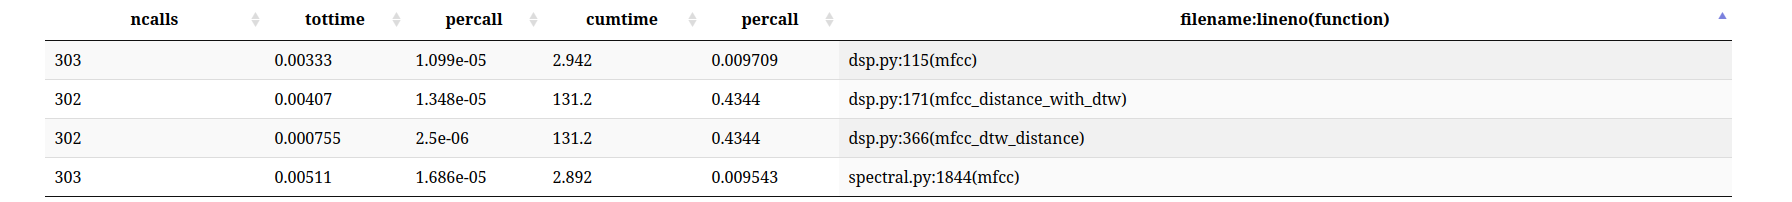
\includegraphics[width=1.0\linewidth]{rys07/mfcc_search.png}
    \caption{
      Porównanie czasu obliczania współczynników MFCC (\texttt{dsp.py:115})
      oraz czasu działania algorytmu DTW (\texttt{dsp.py:171}).
    }\label{fig:mfcc_profiling}
\end{figure}

Rysunki~\ref{fig:target_function_profiling} oraz~\ref{fig:mfcc_profiling}
przedstawiają wyniki profilowania zaimplementowanego algorytmu, wykonane
za pomocą narzędzia \href{https://jiffyclub.github.io/snakeviz/}{\texttt{snakeviz}}.
W pracy została wykorzystana gotowa implementacja
algorytmu DTW (\textit{dynamic time warping}) w języku \texttt{Python}, której
wykonanie zajmuje największą część czasu obliczania wartości funkcji celu.
Wykorzystanie pakietu numerycznego \texttt{numpy} bądź implementacja DTW w
kompilowanym języku programowania może znacząco poprawić szybkość działania algorytmu.

\section{Potencjalne drogi dalszego rozwoju algorytmu}\label{sec:potential_improvements}

Pierwszym krokiem, który należy wykonać w celu usprawnienia
algorytmu optymalizacji jest przygotowanie zbioru dźwięków,
które będą służyły za \textbf{zbiór weryfikujący poprawność działania algorytmu}.
Przykłady zaczerpnięte z literatury~\cite{evolutionary_puredata_results}
nie zawierają wystarczająco bogatej gamy możliwych do wygenerowania
barw dźwięku, które wymusiłyby na algorytmie optymalizacji wykorzystanie
różnorodnych algorytmów syntezy i struktur grafu DSP\@. Wyniki
eksperymentów wykonanych w rozdziale~\ref{chap:research} pozwalają
na zasugerowanie zbioru cech dźwięków, których warianty
powinny być zawarte w zbiorze weryfikującym:

\begin{enumerate}
  \item Typ syntezy:
  \begin{itemize}
    \item synteza \textit{analog modeling},
    \item synteza FM,
    \item synteza \textit{physical modeling}.
  \end{itemize}
  \item Dynamika dźwięku:
    \begin{itemize}
      \item Głośny od samego początku, dynamicznie słabnący,
      \item Równomiernie głośny przez całą długość nagrania,
      \item Powoli narastający i powoli słabnący.
    \end{itemize}
\end{enumerate}

% Po przygotowaniu zbioru walidacyjnego

% Podczas implementacji algorytmu optymalizacji grafu oraz prowadzenia badań

\subsection{Rozmiar okna w algorytmie DTW}

W domyślnym wariancie, algorytm DTW przeszukuje cały sygnał
przy poszukuwaniu pasujących do siebie segmentów. Takie
zachowanie zwiększa złożoność czasową algorytmu, jednocześnie
zmniejszając karę za niedokładne odwzorowanie zmian w dynamice dźwięku.
Przeprowadzone w ramach pracy testy pozwalają sugerować, że zmniejszenie
rozmiaru okna w algorytmie DTW pozwoli na jednoczesne przyspieszenie czasu
wyliczania funkcji celu i usprawni wyniki optymalizacji.

  % \item Różne wielkości okna DTW,
\subsection{Lepsza reprezentacja struktury grafu DSP w genotypie}

Jak opisano w sekcji~\ref{sec:graph_structure_definition}, genotyp grafu DSP
podzielony jest na dwa fragmenty:

\begin{itemize}
  \item $S$ -- fragment odpowiadający za strukturę grafu,
  \item $P$ -- fragment odpowiadający za wartości parametrów w grafie.
\end{itemize}

Po wygenerowaniu danej struktury grafu $G_s$~(\ref{eq:graph_structure_generation_function}),
parametry grafu przypisywane są poprzez równoczesne iterowanie przez wektor $P$ oraz
przez listę parametrów w wygenerowanym grafie $G_s$. Zastosowanie takiego algorytmu
powoduje, że zmiana struktury grafu może spowodować przypisanie parametrów w inne miejsca
na nowym grafie, gdzie ich wartości będą miały zupełnie inny wpływ na sygnał
generowany przez graf. Problem można rozwiązać poprzez trwałe przypisanie danych
parametrów $p_i$ do konkretnych parametrów konkretnej struktury w grafie. Jeśli gen 
tworzący daną strukturę nie będzie aktywny, geny określające parametry tej struktury nie będą
miały wpływu na generowany sygnał i nie zaburzą sposobu przypisania pozostałych genów.


\subsection{Dalsze poszukiwania funkcji celu porównującej barwę sygnałów dźwiękowych}

W pracach przeanalizowanych podczas przeglądu literatury wykorzystano 2 podejścia
do porównania barwy sygnałów dźwiękowych: różnica między spektrogramami oraz
różnica między wartościami współczynników MFCC
(szczegóły opisano w rozdziale~\ref{target_function_chapter}).
Wyniki przeglądu literatury pozwalają podejrzewać, że porównywanie sygnałów
dźwiękowych pod względem ich barwy w kontekście brzmienia muzycznego
nie jest szeroko zbadanym problemem i istnieje potencjał na opracowanie
nowych rozwiązań.


\subsection{Trenowanie na coraz dłuższych fragmentach dźwięku}

Ponieważ złożoność czasowa algorytmu DTW wynosi $O(N^2/\log\log N)$~\cite{dtw_time_complexity},
im dłuższy jest zadany sygnał dźwiękowy, tym bardziej czas wyliczenia
wartości funkcji celu dominuje nad czasem syntezy sygnału dźwiękowego. Potencjalnym
rozwiązaniem tego problemu jest podzielenie optymalizacji na etapy, w których
do optymalizacji grafu DSP wykorzystywane są coraz dłuższe fragmenty dźwięku docelowego.

\subsection{Rozszerzenie genotypu grafu DSP o dodatkowe źródła modulacji}

W syntezatorach dźwięku często wykorzystuje się sygnały modulujące (przedstawione
na rysunkach~\ref{fig:mother32} oraz~\ref{fig:minilogue_diagram}), które modulują
dane parametry generowanego sygnału za pomocą sygnałów kontrolnych (CV). 
W pracy wykorzystano jedynie sygnał obwiedni (\textit{ADSR envelope}),
modulujący intensywność modulacji w przypadku syntezy FM~(\ref{fig:gene_f1})
lub częstotliwość odcięcia w przypadku syntezy
\textit{analog modeling}~(\ref{sec:filters_selection_graph_structure}).
Rozszerzenie zbioru dostępnych sygnałów kontrolnych o oscylator niskoczęstotliwościowy
(\textit{LFO - low frequency oscillator}), który w zależności od genotypu
moduluje różne parametry w grafie DSP może znacząco zwiększyć różnorodność
generowanych barw dźwięku.


\section{Subiektywna natura porównania}

Generowanie dźwięku stanowi zagadnienie,
które w dużej mierze zależy od subiektywnego odbioru słuchaczy.
Ocena zgodności barwy dźwięku dźwięku według określonej funkcji celu
niekoniecznie przekłada się na subiektywną preferencję użytkownika.
Istnieje możliwość, że niedoskonałości funkcji celu mogą wpływać korzystnie na 
odbiór przez słuchaczy, ponieważ dostarczą nieoczekiwanych efektów, 
które mogą być wykorzystane jako źródło inspiracji w procesie kreatywnym.
